%% $Id: louveaux-epfl06.tex,v 1.5 2006/07/10 13:46:20 louveaux Exp $
%%\documentclass[9pt,trans]{beamer}
\documentclass[10pt,handout]{beamer}
\usepackage{beamerfoils}%% FoilTeX emulation
\usepackage{epsfig}
\usepackage{eurosym}
\mode<presentation>
{
  \usetheme{Boadilla}
  % oder ...

  \setbeamercovered{transparent}
  % oder auch nicht
}
\usepackage[french]{babel}
\usepackage[latin1]{inputenc}
%%\usepackage{times}
%%\usepackage[T1]{fontenc}
%\usepackage{booktabs}

%%\includeonlyframes{current}

\title{Discrete Optimization}

\author{Quentin
Louveaux}
\date{2016}
\institute{ULg - Institut Montefiore}

% Falls eine Logodatei namens "university-logo-filename.xxx" vorhanden
% ist, wobei xxx ein von latex bzw. pdflatex lesbares Graphikformat
% ist, so kann man wie folgt ein Logo einf|gen:

% \pgfdeclareimage[height=0.5cm]{university-logo}{university-logo-filename}
% \logo{\pgfuseimage{university-logo}}

% Folgendes sollte gelvscht werden, wenn man nicht am Anfang jedes
% Unterabschnitts die Gliederung nochmal sehen mvchte.
%% \AtBeginSection[]
%% {
%%   \begin{frame}<beamer>
%%     \frametitle{Gliederung}
%%     \tableofcontents[currentsection,currentsubsection]
%%   \end{frame}
%% }

% Falls Aufzdhlungen immer schrittweise gezeigt werden sollen, kann
% folgendes Kommando benutzt werden:

\beamerdefaultoverlayspecification{<+->}

%%%%%%
\definecolor{rot}{rgb}{1,0,0}
\definecolor{gruen}{rgb}{0,1,0}
\definecolor{blau}{rgb}{0,0,1}

%%% number sets
\newcommand{\Z}       {\mathbb{Z} }
\newcommand{\R}       {\mathbb{R} }
\newcommand{\Q}       {\mathbb{Q} }
\newcommand{\N}       {\mathbb{N} }
\newcommand{\spa}     {\text{span}}
\newcommand{\lin}     {\text{span}}
\newcommand{\inter}   {\text{int} }


%%% mathematical stuff
\newcommand{\sosR}    {\sum^2}
\newcommand*{\transpose}[1]  { {#1}^T }
\newcommand*{\rounddown}[1]  {\left\floor #1 \right\rfloor}
\newcommand*{\roundup}[1]    {\left\lceil  #1 \right\rceil}
\newcommand*{\ipart}[1]      {\rounddown{#1}}
\newcommand*{\fpart}[1]      {\mathfrak{f}\left(#1\right)}


\newcommand*{\iepoly}[2]  {z_{#1}\left(#2\right)}
\newcommand*{\redmon}[3]  {r_{#1}^{#2}\left( #3 \right)}
\newcommand*{\redset}[1]  {#1^{\emph{red}}}

\newcommand*{\Gpoly}[1] {P_{[#1]}}

\newcommand*{\nonc}[1]{\overline{#1}}
\newcommand*{\const}[1]{#1_0}

\newcommand{\define}{\stackrel{\rm def.}{\Leftrightarrow}}
\newcommand{\qform}[3]{\frac{1}{2} x^{\top}#1x + #2^{\top}x + #3}
\def\xzero{x^{0}}
\newcommand{\gxh}[2]{{g_{#1}(#2)}}

\def\pcone_k{{\mathcal C}_{k}(f)}
\def\orthant_j{{\mathcal O}_{j}}

\def\BDB{BDB^{\top}}
\def\LDL{LDL^{\top}}
\def\bA{A}
\def\bb{b}
\def\bc{c}
\def\bh{h}
\def\bp{p}
\def\bx{x}
\def\by{y}
\def\bu{u}
\def\bv{v}
\def\bd{d}
\def\T{^{T}}
\def\D{}
\def\mb{{\bf}}
\def\sep{}
\def\bo{0}
\def\bw{w}
\def\ba{a}
\def\bg{g}
\def\bH{H}
\def\be{e}

\let\ve=\relax
\newcommand\vealpha{{\alpha}}
\newcommand{\st}{\mathrm{s.t.}}
\DeclareMathOperator\conv{conv}
\DeclareMathOperator\cone{cone}
\newcommand{\B}{\{0,1\}}

\newcommand*{\person}[1] {\textsc{#1}}

\newtheorem{algorithm}{Algorithmus}

\makeatletter
\newenvironment{rmat}{\left(\null\,\vcenter\bgroup
  \Let@\restore@math@cr\default@tag
  \baselineskip6\ex@ \lineskip1.5\ex@ \lineskiplimit\lineskip
  \ialign\bgroup\hfil$\m@th\scriptstyle##$&&\thickspace
  \hfil$\m@th\scriptstyle##$\crcr
}{%
  \crcr\egroup\egroup\,\right)%
}
\makeatother

%%%%%%%%%%%%%%%%%%%%%%%%%%%%%%%%%%%%%%%%%%%%%%%%%%%%%%%%%%%%%%%%%%%%%%%%%%%%%%%%
%\begin{frame}
  %\titlepage
%\end{frame}

%% \begin{frame}
%%   \frametitle{Gliederung}
%%   \tableofcontents
%%   % Die Option [pausesections] kvnnte n|tzlich sein.
%% \end{frame}


%%%%%%%%%%%%%%%%%%%%%%%%%%%%%%%%%%%%%%%%%%%%%%%%%%%%%%%%%%%%%%%%%%

\definecolor{orange}{rgb}{0.8,0.3,0.0}
\definecolor{darkgreen}{rgb}{0.0,0.5,0.0}
\definecolor{gold}{rgb}{1.0,0.8,0.0}
\definecolor{brown}{rgb}{0.6,0.2,0.2}
\definecolor{blue4}{rgb}{0,0,144}
\definecolor{white}{rgb}{255,255,255}
\definecolor{blueexample}{rgb}{0.2,0.2,0.7}
\begin{document}
\begin{frame}
  \titlepage
\end{frame}
\begin{frame} \frametitle{Dynamic Programming}
  \begin{itemize}
  \item Dynamic Programming (DP) is an algorithm for combinatorial
    problems having the ``optimal substructure property.''
  \item It solves a sequence of \alert{subproblems} where each subproblem \alert{capitalizes} on
    the solution of the previous subproblems
  \item This is different from divide and conquer
    (e.g. branch-and-bound) which is a top-down approach that splits the
    problem in disjoint subproblems, and compares their solutions.
  \item In DP, subproblems overlap: each subproblem \alert{contains} the previous subproblems.
  \end{itemize}
\end{frame}

\begin{frame} \frametitle{Example: shortest path.}
  \begin{center}
    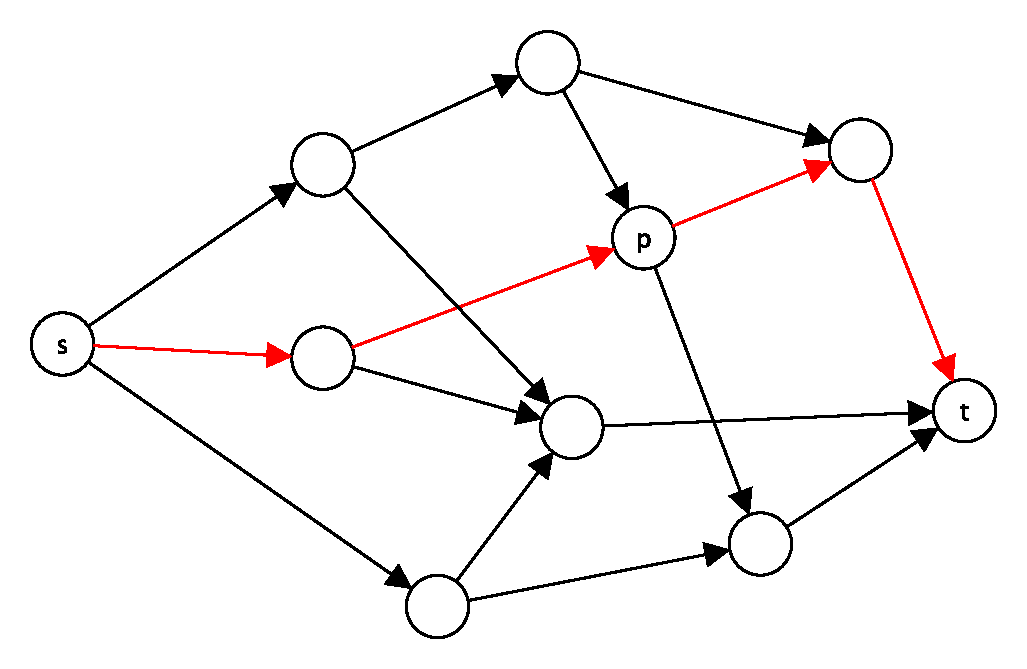
\includegraphics[width=0.6\textwidth]{SP.pdf}
  \end{center}


        \begin{itemize}
        \item If an optimal path from $s$ to $t$ goes through $p$
        \item then it contains the optimal path from $s$ to $p$ and the optimal path from $p$ to $t$.
        \end{itemize}

\end{frame}

\begin{frame} \frametitle{Theorem of optimality (Bellman)}
  \begin{center}
    \alert{An optimal policy}
      must contain only optimal sub-policies
    or \\ [10mm]
    a policy is optimal if, at a stated stage, whatever the
      preceding decisions have been, the decisions still to be taken
      constitute an optimal policy when the result of the previous
      decisions is included.
  \end{center}
  % \item Example. Benefits and disadvantages.
\end{frame}

%\begin{frame} \frametitle{Definitions}
%  \begin{itemize}
%  \item Stage $t$: an opportunity to take a decision (not
%    necessarily a time period)
%  \item Decision $x_t$ (or action, or transition): an optimization
%    variable in the usual sense.
%  \item State $s_t$: summary of the system, given the decisions that
%    were already taken. In a Markovian setting, $s_{t+1} = f(s_t, x_t)$.
%  \item Value function $H(s_t)$: assigns a value to a state (e.g. cost-to-go).
%  \item State-action value function $Q(s_t,x_t)$: value of taking a decision in a
%    given state. $$H(s_t) = \max_{x_t} Q(s_t,x_t)$$
%  \end{itemize}
%\end{frame}
%
\begin{frame} \frametitle{Numerical example: shortest path.}
  \begin{columns}
    \begin{column}{0.4\textwidth}
      {\small Example:\\ Optimal path from A to J: ACHJ.
        \begin{itemize}
        \item ACH is the optimal path from A to H.
        \item CHJ is the optimal path from C to J.
        \end{itemize}}
    \end{column}
    
    \begin{column}{0.5\textwidth}
      
      \begin{figure}[H]
        \centering
        \includegraphics[width=\textwidth]{DPexample.pdf}
        % \caption{DP example.}
        \label{fig:DPexample}
      \end{figure}
    \end{column}
  \end{columns}
\end{frame}

\begin{frame} \frametitle{Guidelines for applying DP}
  \begin{itemize}
  \item View the choice of a feasible solution as a sequence of
    decisions occuring in stages, and so that the total cost is the
    sum of the costs of individual solutions.
  \item Define the state as a summary of all relevant past decisions.
  \item Determine which state transitions are possible, i.e. which
    decision can / cannot be taken in each state (hence the cost
    of a transition is the cost of the corresponding decision).
  \item Write a recursion on the optimal cost from the origin state to
    a destination state. Solving this recursion gives you the optimal cost.
  \item If needed, keep information on the optimal path from the origin state to
    a destination state (to ease reconstruction of the solution).
  \end{itemize}
\end{frame}

\begin{frame}\frametitle{Example: uncapacitated lot sizing}
  \begin{center}
    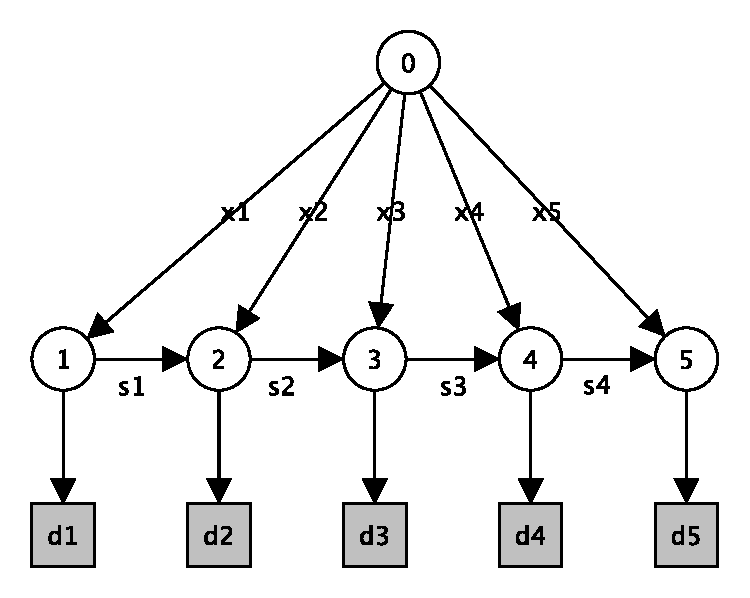
\includegraphics[width=0.6\textwidth]{LotSizingNetwork.pdf}
  \end{center}

\begin{itemize}
\item MIP formulation
\item Analysis of the solutions
\item DP recursion equation
\item Numerical example 
\end{itemize}
\end{frame}

\begin{frame}\frametitle{Example: Binary Knapsack}
\begin{itemize}
\item MIP formulation.
\item DP recursion equation.
\item Complexity.
\item Numerical example.
\end{itemize}
\end{frame}

\begin{frame}\frametitle{Example: Integer Knapsack}
\begin{itemize}
\item MIP formulation
\item DP recursion equation.
\item Complexity.
\item Numerical example.
\end{itemize}
\end{frame}



\begin{frame} \frametitle{Many diverse applications of DP}
  \begin{itemize}
  \item Multiply several matrices while performing the fewest total scalar multiplications.
  \item Find the longest common subsequence of two sequences (Protein
    sequences alignment).
  \item Construct binary search trees that are optimal, given a known distribution of keys to be looked up.
  \item The Viterbi algorithm (cf. Information Theory course) is a DP algorithm.
  \item Central role in the Reinforcement Learning paradigm (cf. Applied Inductive Learning course).
  \end{itemize}
\end{frame}
\end{document}
